\documentclass[10pt]{report}

\usepackage{talks}
\newcommand{\expect}[1]{\mathbb{E}\!\left[ #1 \right]}
\newcommand{\reals}{\mathbb{R}}
\newcommand{\draw}[2]{#1^{(#2)}}
\usepackage{mathpazo}
  \renewcommand{\baselinestretch}{1.05}
\usepackage{sourcecodepro}
\usepackage{tikz}
  \usetikzlibrary{arrows.meta, angles, quotes, calc, positioning, shapes}
\usepackage{lastpage}
\usepackage{fancyhdr}



\pagestyle{fancy}
\fancyhf{}
\fancyfoot[C]{\footnotesize \sf{\thepage}/\pageref{LastPage}}
\setlength{\footskip}{9pt}
\thispagestyle{empty}

\newcommand{\ddfrac}[2]{\frac{\strut \displaystyle #1}{\strut \displaystyle #2}}
\newcommand{\pos}[2]{#1^{(#2)}}


\begin{document}
\sf
\mbox{ } \\
\spc{\LARGE\bfseries \color{MidnightBlue}{GIST: Gibbs self-tuning for HMC}}
\\[12pt]
\noindent 
\spc{\large\bfseries \color{MidnightBlue}{Bob Carpenter}}
\\[2pt]
\spc{\small Center for Computational Mathematics}
\\[-1pt]
\spc{\small Flatiron Institute}
\\[2pt]
\spc{\footnotesize \url{bcarpenter@flatironinstitute.org}}
\\[12pt]
\spc{\small with \ \myemph{Nawaf Bou-Rabee} (Rutgers), \myemph{Tore Kleppe} (Stavanger), \myemph{Milo Marsden}
  (Stanford)}
\noindent
\\
\vfill
\noindent\spc{\footnotesize October 2024 \qquad Yale FDS Sampling Worskhop}
\hfill

\includegraphics[width=1.5in]{img/flatiron-logo.png}

\sld{Where are we going?}
\begin{itemize}
\item A new {framework} for
  \myemph{locally tuning} Hamiltonian Monte Carlo (HMC)
  \begin{subitemize}
    \item (a) {number of steps}, (b) {step size}, (c) {mass matrix}
    \end{subitemize}
\item \myemph{Tuning parameters} are \myemph{Gibbs sampled} given
  position and momentum.
\item Metropolis-Hastings \myemph{accept probability} adjusted for balance.
\item \myemph{Warmup} (global, non-Markovian) is \myemph{not required}.
\begin{subitemize}
\item still \myemph{need burn in} to find bulk of probability mass
\end{subitemize}
\item \myemph{Simplifies proofs} of correctness for instances
  \begin{subitemize}
    \item e.g., randomized HMC, NUTS, multinomial HMC,
      apogee-to-apogee, etc.
    \end{subitemize}
\end{itemize}

\sld{Hamiltonian dynamics}
\begin{itemize}
\item \myemph{Auxiliary variable}: couple \myemph{momentum} $\rho \in
  \mathbb{R}^D$ with \myemph{position} $\theta \in \mathbb{R}^D$
\item \myemph{Potential energy}: $U(\theta) = -\log p(\theta \mid y)$
\item \myemph{Kinetic energy}: $K(\rho) = -\log \textrm{normal}(\rho
  \mid 0, M) = -\frac{1}{2} \cdot \rho^{\top} \cdot M^{-1} \cdot
  \rho + \textrm{const.}$
\item \myemph{Hamiltonian}: $H(\theta, \rho) = U(\theta) + K(\rho)$
\item \myemph{Dynamics} (time-independent):
  \begin{align*}
  \nabla_\theta \, H(\theta, \rho) &= \rho
  \\[4pt]                                     
  \nabla_\rho \, H(\theta, \rho) &= -\nabla_{\theta} \, \log
  p(\theta \mid y)
  \end{align*}
  \item \myemph{Joint density}: $\log p(\theta, \rho) = \log p(\theta \mid y) + \log \textrm{normal}(\rho \mid 0, 1) = -H(\theta, \rho)$
\end{itemize}

\sld{Leapfrog algorithm: $\Phi_{\epsilon, M}$}
\begin{itemize}
\item \myemph{Explicit solver} for Hamiltonian dynamics (given initial state).
\item \myemph{Given} log density $\log p(\theta)$, step size
  $\epsilon$, positive definite mass matrix $M$, 
\item \myemph{Leapfrog step}: $\Phi_{\epsilon, M}(\theta, \rho) = \theta'', \rho''$, where
  \begin{subitemize}
    \item a. $\rho' = \rho + \frac{\epsilon}{2} \cdot \nabla \log p(\theta \mid y)$
    \item b. $\theta'' = \theta + \frac{\epsilon} \cdot M^{-1} \cdot \rho'$
    \item c. $\rho'' = \rho' + \frac{\epsilon}{2} \cdot \nabla \log p(\theta' \mid y)$
    \end{subitemize}
\item \myemph{Multiple steps}: $\Phi^0_{\epsilon, M}$ is the
  identity; \quad $\Phi^{t + 1}_{\epsilon, M} = \Phi^t_{\epsilon,M} \circ
  \Phi_{\epsilon,M}$
\item \myemph{Error}: one-step $\mathcal{O}(\epsilon^3)$; more than
  one step $\mathcal{O}(\epsilon^2)$ (!)
\end{itemize}

\sld{HMC Markov transition}
\begin{itemize}
\item \myemph{Input}:
  \begin{subitemize}
  \item {position} $\theta$
  \item {step size} $\epsilon > 0,$
  \item {number of steps} $T \in \mathbb{N}$
  \item {mass matrix} $M$ (symmetric positive definite)
  \end{subitemize}
\item \myemph{Refresh momentum}: Gibbs sample $\rho \sim \textrm{normal}(0, M)$
\item \myemph{Simulate dynamics}:  Let $\theta^*, \rho^* = \Phi_{\epsilon,M}^T(\theta, \rho)$
\item \myemph{Metropolize}: Return $\theta^*$ if $\textrm{uniform}(0, 1) <
  \dfrac{p(\theta^*, \rho^*)}
       {p(\theta, \rho)}$ else return $\theta$
\end{itemize}

\sld{HMC tuning hard: 1000D standard normal}
\begin{subitemize}
\item step size ($x$-axis) vs.\ ESS $y$-axis; HMC (top), randomized
  steps HMC (bottom), NUTS (dashed); 
  4/16/64 steps (facets); $\mathbb{E}[\theta]$ (blue) and
  $\mathbb{E}[\theta^2]$ (red)
\end{subitemize}
\vspace*{-3pt}
\begin{center}
  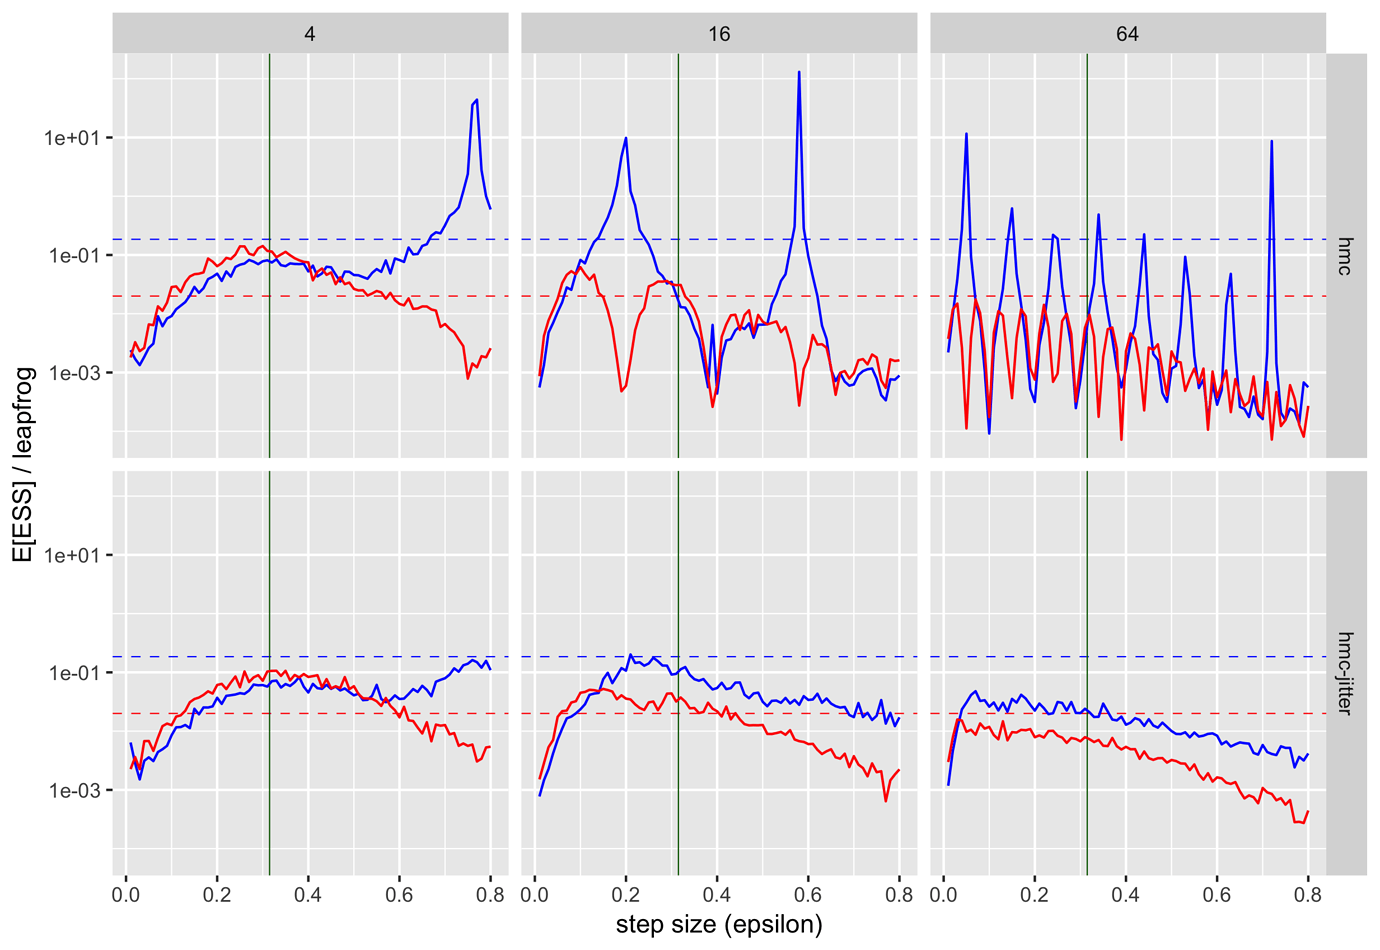
\includegraphics[width=2.6in]{img/hmc-harmonics.png}
\end{center}

\sld{Gibbs self tuning (GIST)}
\begin{itemize}
\item \myemph{Couple tuning} parameters $\alpha$ (step
  size, number of steps, mass matrix)
\item \myemph{Free choice} of conditional tuning-parameter distribution $p(\alpha \mid \theta, \rho)$
\item Each iteration, \myemph{Gibbs sample} $\alpha^* \sim p( \cdot \mid \theta,
  \rho)$
\item \myemph{Propose} $\theta^*, \rho^* = \Phi^{T^*}_{\epsilon^*,
    M^*}(\theta, \rho)$ given $\alpha^* = \epsilon^*,
  M^*, T^*$
\item Metropolis-Hastings \myemph{accept probability}:
  $$
  1 \wedge
  \dfrac{p(\theta^*, \rho^*)}
  {p(\theta, \rho)}
  \cdot
  \dfrac{p(\alpha^* \mid \theta^*, \rho^*)}
       {p(\alpha^* \mid \theta, \rho)}
       $$
\item Straightforward to establish \myemph{detailed balance}.
\end{itemize}

\sld{Randomized HMC is GIST}
\begin{itemize}
\item HMC works with \myemph{randomized tuning} (e.g., steps $L$ or
  step size $\epsilon$)
\item Other tuning parameters are fixed (i.e., delta function distributions)
\item \myemph{Randomizing} step size or number of steps \myemph{removes
    harmonics} that plague HMC with fixed step size and steps, e.g.,
  $$p(L \mid \theta, \rho) = \textrm{uniform}(L \mid 1, N).$$
\item If tuning parameter distribution does \myemph{not depend on position or
  momentum}, then $p(\alpha^* \mid \theta, \rho) = p(\alpha^* \mid \theta^*,
  \rho^*)$, and thus
  $$
  1 \wedge
  \dfrac{p(\theta^*, \rho^*)}
       {p(\theta, \rho)}
  \cdot
  \dfrac{p(\alpha^* \mid \theta^*, \rho^*)}
       {p(\alpha^* \mid \theta, \rho)}
       =
       1 \wedge
       \dfrac{p(\theta^*, \rho^*)}{p(\theta, \rho)}
  $$       
\end{itemize}

\sld{Multinomial HMC is GIST}
\begin{itemize}
\item Multinomial HMC fixes \myemph{steps} $L$, step size
  $\epsilon$, mass matrix $M$.
\item Each iteration, take $F \sim \textrm{uniform}(0, L)$ \myemph{forward
    steps} and $B = L - F$ \myemph{backward steps}.
  \begin{subitemize}
  \item Let $\Phi^{-n}_{\epsilon, M}(\rho, \tau)
    = \Phi^{n}_{\epsilon, M}(\rho, -\tau)$ (i.e., \myemph{flip
      momentum})
    \end{subitemize}
  \item \myemph{Generate number of steps} with probability
    $$p(n) \propto p(\theta(n), \rho(n))$$ from
    candidates  $\theta(n), \rho(n) = \Phi^n_{\epsilon,
      M}(\theta, \rho)$, where $n \in \{ -B, -B + 1, \ldots, 0, 1, \ldots, F \}$
\item GIST \myemph{acceptance probability is 100\%}!
\end{itemize}

\sld{Proof sketch of multinomial 100\% acceptance}
\begin{itemize}
\item Without loss of generality, assume selected $n > 0$
% \item GIST \myemph{acceptance probability} is
%   $\dfrac{p(\theta(n),\,   \rho(n))}
%        {p(\pos{\theta}{0},\, \pos{\rho}{0})}
%   \cdot
%   \dfrac{p(n \, \mid \, \theta(n),\, -\rho(n))}
%        {p(n \, \mid \, \pos{\theta}{0},\, \pos{\rho}{0})}$
\item Set of length $L$ trajectories from 0 to $n$ same
  as set from $n$ to 0, hence
\begin{align*}
  p(n \mid \pos{\theta}{0}, \pos{\rho}{0})
  &= \sum_{i=0}^{L-n}
      \dfrac{p(\pos{\theta}{n},\, \pos{\rho}{n})}
            {\sum_{j=i}^{i + L} p(\theta(j),\, \rho(j))}
  &= p(\pos{\theta}{n},\, \pos{\rho}{n}) / Z
  \\[4pt]
  p(n \mid \theta(n),\, -\rho(n))
  &= \sum_{i=0}^{L-n} \dfrac{p(\pos{\theta}{0},\, \pos{\rho}{0})}
                           {\sum_{j=i}^{i + L} p(\theta(j),\, \rho(j))}
  & = p(\pos{\theta}{0},\, \pos{\rho}{0}) / Z
\end{align*}
\item \myemph{Correction} for detailed balance is thus
$\dfrac{p(\pos{\theta}{0},\, \pos{\rho}{0})}
      {p(\theta(n),\, \rho(n))}$
\item The correction is \myemph{inverse of Metropolis}, so \myemph{acceptance is 100\%}.
\end{itemize}

% \sld{Multinomial path similarity illustration}
% \begin{itemize}
% \item Trajectories \myemph{starting at $0$} and \myemph{including $N$}
% \end{itemize}
% \begin{verbatim}
%      F = L,   B = 0:             0 ... N ...        L

%      F = L-1, B = 1:          -1 0 ... N ... (L-1)

%         .                           .
%         .                           .
%         .                           .

%      F = N, B = L-N:  -(L-N) ... 0 ... N
% \end{verbatim}
% \begin{itemize}
% \item are \myemph{identical} to trajectories \myemph{starting at $N$}
%   and \myemph{including $0$} (flip F \& B)
% \end{itemize}

\sld{NUTS, AAPS, and autoMALA are GIST samplers}
\begin{itemize}
\item Original and revised \myemph{no-U-turn sampler} (NUTS) are GIST samplers.
\item The \myemph{apogee-to-apogee path
    sampler} (AAPS) is a GIST sampler.
\item Cast as conditional \myemph{distributions on number of steps} given
  current position and momentum with a \myemph{multinomial acceptance}.
\item The \myemph{autoMALA sampler} is a GIST sampler for step size. 
\vfill
\item There are detailed \myemph{proofs in the paper} for AAPS and NUTS. 
\end{itemize}

\sld{Alternative to NUTS}
\begin{itemize}
\item \myemph{First GIST paper} ({\slshape arXiv}) includes \myemph{novel alternative to NUTS}:
  \begin{subitemize}
  \item Evolve trajectory in one direction until U-turn.
  \item Select point randomly along trajectory.
  \item Evaluate reverse trajectory until U-turn.
  \item Adjust acceptance with GIST condition.
  \end{subitemize}
\item \myemph{Biasing toward later states} helps (like NUTS, AAPS).
\item \myemph{Performance comparable to NUTS} on a range of problems.
\item Could improve w.\ selection \myemph{proportional to density} (like NUTS, AAPS).
\end{itemize}

\sld{Step size adaptation 1: max $\tau$-stable step size}
\begin{itemize}
\item Find \myemph{largest step size} in a schedule that \myemph{conserves Hamiltonian} to within $\tau$ between all states on trajectory.
\item Fix mass matrix $M$, steps $L$, \myemph{maximum step size}
  $\epsilon^\text{max}$, \myemph{error tolerance} $\tau$
\item Define a function $\textrm{\bfseries stepReduce}(\theta, \rho, M, L, \epsilon^\text{max}, \tau)$ as follows.
\begin{enumerate}
  \item Let $\epsilon = \epsilon^\text{max}$
  \item While $\textrm{max}_{\normalsize 1 \leq m, n \leq L}(H \circ \Phi^m_{\epsilon, M}(\theta, \rho) - H \circ \Phi^n_{\epsilon,M}(\theta, \rho))) > \tau$:
    \begin{itemize}
    \item let $\epsilon = \epsilon / 2$
    \end{itemize}
  \item Return $\epsilon$.
\end{enumerate}
\end{itemize}

\sld{Step size adapation 2: GIST HMC}
\begin{itemize}
\item Given everything (state, mass matrix, steps, max step size, error tolerance),
  \begin{enumerate}
  \item Let $\epsilon^\text{stable} = \text{stepReduce}(\theta, \rho, M, L, \epsilon^\text{max}, \tau)$
  \item Draw $\epsilon \sim \textrm{uniform}\!\left(\left\{ 2^{-1} \cdot \epsilon^\text{stable}, \ \ 2^{0} \cdot \epsilon^\text{stable}, \ \ 2^{1} \cdot \epsilon^\text{stable}\right\}\right).$
  \item Let $(\theta^*, \rho^*) = \Phi^L_{\epsilon, M}(\theta, \rho)$ be the \myemph{proposal}.
  \item Let $\epsilon^* = \text{stepReduce}(\theta, \rho, M, L, \epsilon^\text{max}, \tau)$
  \item Let $\alpha = 1 \wedge \dfrac{p(\theta^*, \rho^*)}{p(\theta, \rho)}
    \cdot
    \textrm{I}\!\left(\epsilon^* \in
      \left\{ 2^{-1} \cdot \epsilon^\text{stable}, \ \ 2^{0} \cdot \epsilon^\text{stable}, \ \ 2^{1} \cdot \epsilon^\text{stable}\right\}
    \right).$
    \item Return $(\theta^*, \rho^*)$ if $\textrm{uniform}(0, 1) < \alpha$, otherwise $(\theta, \rho)$.
    \end{enumerate}
  \item Set $\tau$ so that \myemph{any} $\epsilon^*$ chosen \myemph{is stable}.
  \item Uniform in (2) \myemph{works}, but \myemph{chosen somewhat arbitrarily}.
\end{itemize}

\sld{Step size adaptation 3: GIST NUTS}
\begin{itemize}
\item (1) Replace HMC with \myemph{multinomial HMC} in previous algorithm.
  \begin{subitemize}
  \item Evolve Hamiltonian randomly \myemph{forward and backward} in time $L$ steps.
  \item Select proposal \myemph{propto joint density}
  \item GIST \myemph{acceptance 100\%} if \myemph{adapted step sizes compatible}.
  \end{subitemize}
\item (2) Replace multinomial with \myemph{multinomial NUTS}. \begin{subitemize}
  \item Just like (1), but challenging to write down on slide (and paper).
  \item GIST \myemph{acceptance still 100\%} if adapted step sizes compatible.
  \item See \myemph{second GIST paper} on {\slshape arXiv} (ref at end).
\end{subitemize}
\end{itemize}

\sld{Neal's funnel}
\begin{itemize}
\item Radford \myemph{Neal's funnel} is a \myemph{hierarchical} regression with \myemph{no data}
  $$\textstyle
  p(\beta, \alpha) = \textrm{normal}(\beta \mid 0, 3) \cdot \prod_{d=2}^D \textrm{normal}(\alpha_d \mid 0, \exp(\beta / 2))
  $$
  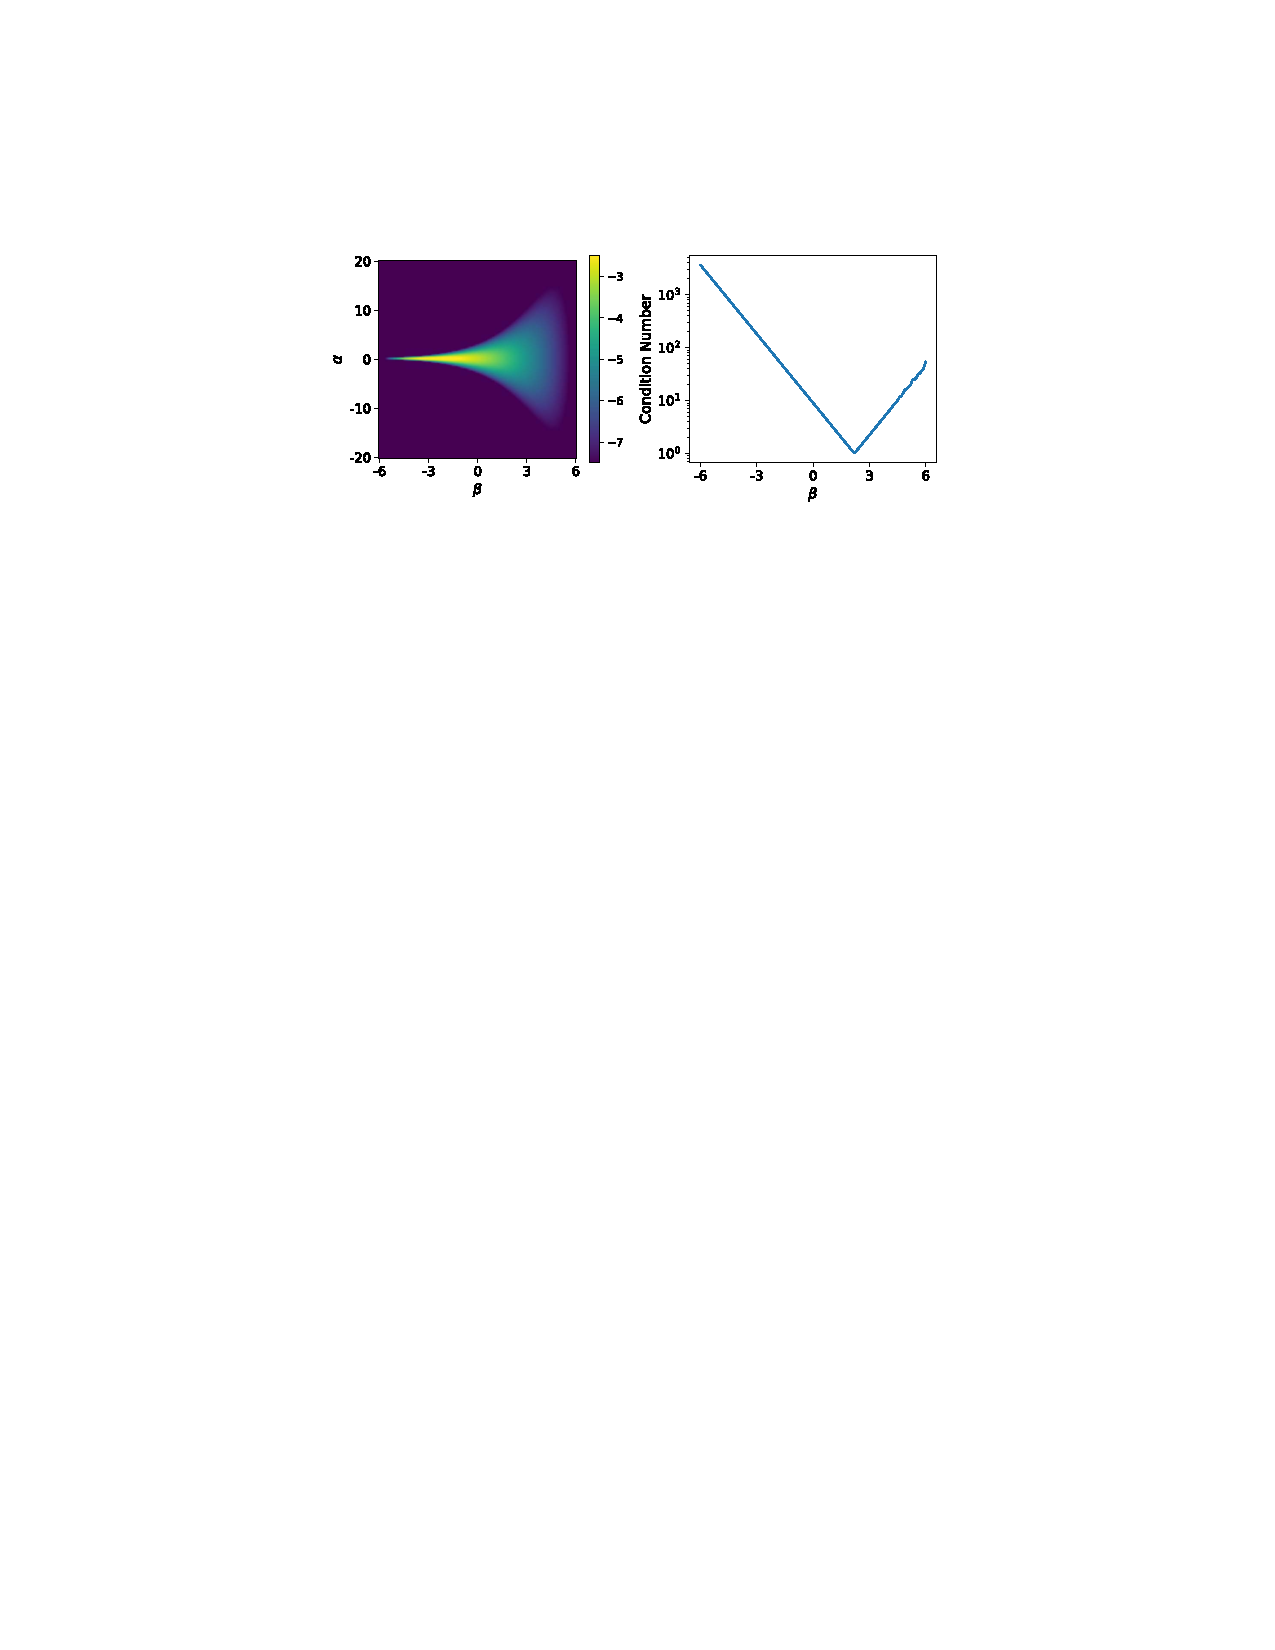
\includegraphics[width=0.6\textwidth]{funnel-condition.pdf}
  \quad 
  \begin{minipage}[t]{1in}
    \vspace*{-1in}
    \small Condition measured vs. central 95\% of $\beta$, with all $\alpha_i = 0$
  \end{minipage}

\item \myemph{Very challenging} in mouth/neck due to varying scale (eigenvalues/vectors).
\end{itemize}
  
\sld{Empirical evaluation}
\begin{itemize}
\item Histogram of \myemph{marginal posterior} draws for \myemph{log scale $\beta$}
\begin{center}
  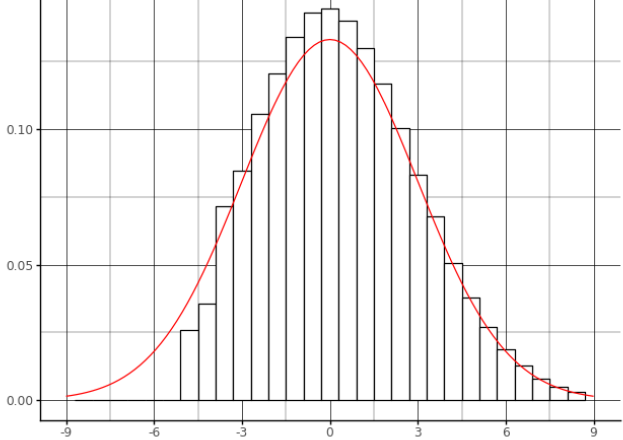
\includegraphics[width=0.4\textwidth]{nuts-funnel.png}
  \quad
  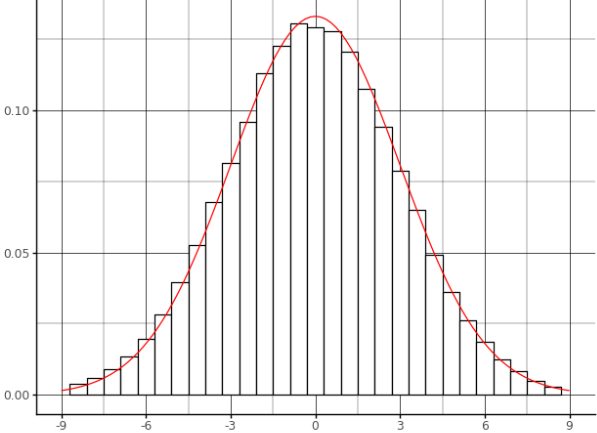
\includegraphics[width=0.4\textwidth]{gist2-funnel.png}
  \\
  \hspace*{0.45in}{\small NUTS \myemph{fails}}\hspace*{1.0in}{\small Adaptive step NUTS \myemph{succeeds}}
\end{center}
\end{itemize}

\sld{Extra work vs.\ NUTS?}
\begin{itemize}
\item NUTS fails funnel, but what about \myemph{cases where NUTS succeeds}?
\item \myemph{Extra work only if} $\text{stepReduce}(\theta, \rho, M, L, \epsilon^\text{max}, \tau) \neq \epsilon^\text{max}$
  \begin{subitemize}
  \item evaluate \myemph{double selected step size} in reverse for stability
  \item if that's stable and not max step size, evauate \myemph{quadruple} selected step size
  \end{subitemize}
\item Randomization scheme bounds work to \myemph{triple} work done by NUTS.
\item Reverse evaluations can be \myemph{parallelized}.
\item \myemph{Extra work only} if NUTS \myemph{diverges on Hamiltonian} beyond threshold $\tau$.
  \begin{subitemize}
  \item Needs \myemph{empirical evaluation} vs.\ NUTS step size adaptation target.
  \end{subitemize}
\end{itemize}

\sld{NUTS with per leapfrog stepsize adaptation}
\begin{itemize}
\item Step size adaptive NUTS is \myemph{suboptimal} in that it
  \begin{subitemize}
  \item uses \myemph{one step size} for \myemph{entire trajectory}
  \item but \myemph{trajectories vary} in \myemph{scale/curvature}
  \end{subitemize}
\item Fix is to \myemph{adapt} step size \myemph{each leapfrog} step.
  \begin{subitemize}
  \item with \myemph{no stepsize randomization}
  \item \myemph{acceptance} involves product of accepting all steps
  \end{subitemize}
\item Restricts \myemph{extra work} (reduced stepsize) to \myemph{where it's needed}
\item \myemph{Works well} on examples we've tried, even w/o stepsize randomization.
\item GIST 3 \myemph{paper in the works}.
\end{itemize}

\sld{Papers and reproducible code}
\begin{itemize}
\item (1) Nawaf Bou-Rabee, Bob Carpenter, and Milo Marsden. 2024. \myemph{GIST: Gibbs 
self-tuning for locally adaptive Hamiltonian Monte 
Carlo}. \textit{arXiv}:2404.15253. 
\item (2) Nawaf Bou-Rabee, Bob Carpenter, Tore Selland Kleppe, Milo Marsden. 2024. \myemph{Incorporating local step-size adaptivity into the no-U-turn sampler using Gibbs self tuning}. \textit{arXiv}:2408.08259.
\vspace*{12pt}  
\item \myemph{GitHub}: \texttt{https://github.com/bob-carpenter/\myemph{adaptive-hmc}}
\vfill 
\item We would \myemph{appreciate feedback} on paper and code.
\end{itemize}

\end{document}

